\documentclass{tufte-handout}
\usepackage{pgfplots}
\usepackage[dvipsnames]{xcolor}
\usepackage{ulem}
\usepackage{subcaption}
\usepackage{amssymb, amsmath, pgfplots, tabularx, siunitx}
\usepackage{algorithm}
\usepackage{algorithmic}
\usepackage{makecell}
\usepackage{amsfonts}
\usepackage{thmtools}
\usepackage{enumitem}
\usepackage{adjustbox}
\usepackage{listings}
\usepackage{booktabs} % Adicionado para tabelas elegantes
\pgfplotsset{compat = newest}

\usepackage{tikz}
\usetikzlibrary{shadings}
\usetikzlibrary{calc,arrows.meta}
\usetikzlibrary{shapes.misc}
\usetikzlibrary{shapes.geometric}
\usetikzlibrary{matrix}
\usetikzlibrary{positioning}
\usetikzlibrary{decorations.pathmorphing} % Adicionado para dendritos sinuosos
\usepackage[most]{tcolorbox}
\usepgfplotslibrary{colormaps,patchplots}

% Cores preservadas
\definecolor{wp-bg}{HTML}{FDF6EF}
\definecolor{wp-text}{HTML}{2D1B0E}
\definecolor{wp-primary}{HTML}{C24A3A}
\definecolor{wp-accent}{HTML}{D4952E}
\definecolor{wp-light}{HTML}{F0DECA}
\definecolor{wp-muted}{HTML}{C4A88A}
\definecolor{wp-dark}{HTML}{1A0F07}
\definecolor{wp-code}{HTML}{FDF2E4}

\pagecolor{wp-bg}
\color{wp-text}

\hypersetup{colorlinks=true,linkcolor=wp-primary,urlcolor=wp-accent}

\let\subsubsection\subsection

% Theorem environments
\declaretheorem[style=plain, name=Definition, numberwithin=section]{defn}
\declaretheorem[style=plain, name=Theorem, numberwithin=section]{thm}
\declaretheorem[style=plain, name=Lemma, numberwithin=section]{lem}
\declaretheorem[style=remark, name=Example, numberwithin=section]{exmp}
\declaretheorem[style=remark, name=Remark, numberwithin=section]{remark}

\tikzset{basic/.style={draw,text width=1em,text badly centered}}
\tikzset{input/.style={basic,circle}}
\tikzset{weights/.style={basic,rectangle}}
\tikzset{functions/.style={basic,circle}}

% Configuração do listings para o mini_nn
\lstdefinestyle{pythonstyle}{
    language=Python,
    backgroundcolor=\color{wp-code},
    basicstyle=\ttfamily\small\color{wp-text},
    keywordstyle=\color{wp-primary}\bfseries,
    stringstyle=\color{wp-accent},
    commentstyle=\color{wp-muted}\itshape,
    numbers=left,
    numberstyle=\tiny\color{wp-muted},
    numbersep=8pt,
    breaklines=true,
    frame=single,
    rulecolor=\color{wp-muted!50},
    framerule=0.5pt,
    xleftmargin=15pt,
    showstringspaces=false
}
\lstset{style=pythonstyle}

\title{Machine Learning Notes \\ Chapter 1: Preliminary Introduction to Deep Learning}
\author{Vitor N. Cabral de Oliveira\\ \href{mailto:vnco@cin.ufpe.br}{vnco@cin.ufpe.br}}
\date{\today}

\begin{document}
\maketitle
\begin{abstract}
    This notebook serves as a comprehensive repository for my Machine Learning studies, with a primary focus on Deep Learning. In this chapter, we establish the foundational concept of mathematical modeling, explore the biological inspiration behind Artificial Neural Networks (ANNs), and formalize their mathematical structure as parametric function approximators.
\end{abstract}

\newpage
\hypersetup{linkcolor=wp-text}
\tableofcontents
\hypersetup{linkcolor=wp-primary}
\newpage

\section{The Concept of Modeling}

Before diving into neurons and weights, we must understand what it means to \textit{model} something. In the physical sciences, a model is a simplified representation of a complex reality. A map is a model of a city; it discards irrelevant details (the color of individual houses) to highlight essential structures (streets and distances). 

In machine learning, we take a formal approach. We assume there is a true, underlying relationship between some input variables $\mathbf{x}$ and an output $y$. We cannot observe this relationship directly, but we can observe a dataset $\mathcal{D} = \{(\mathbf{x}_d, y_d)\}_{d=1}^N$. 

\begin{marginfigure}[-2.0cm]
\centering
\resizebox{0.97\marginparwidth}{!}{%
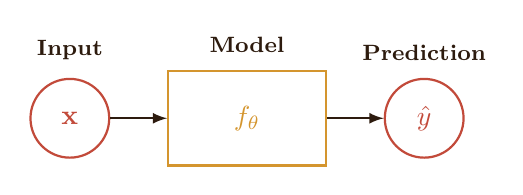
\begin{tikzpicture}[scale=0.9, >=latex, node distance=1.5cm]
    \node[draw, circle, wp-primary, thick, minimum size=1cm] (x) at (0,0) {$\mathbf{x}$};
    \node[draw, rectangle, wp-accent, thick, minimum width=2cm, minimum height=1.2cm] (model) at (2.5,0) {$f_\theta$};
    \node[draw, circle, wp-primary, thick, minimum size=1cm] (y) at (5,0) {$\hat{y}$};
    \draw[->, thick, wp-text] (x) -- (model);
    \draw[->, thick, wp-text] (model) -- (y);
    \node[wp-text, font=\footnotesize\bfseries, above=0.1cm of x] {Input};
    \node[wp-text, font=\footnotesize\bfseries, above=0.1cm of model] {Model};
    \node[wp-text, font=\footnotesize\bfseries, above=0.1cm of y] {Prediction};
\end{tikzpicture}}
\caption{The standard ML pipeline: a model $f_\theta$ maps inputs to outputs.}
\label{fig:modeling_pipeline}
\end{marginfigure}

\begin{defn}[Mathematical Model]
A mathematical model is a parametric function $f_\theta: \mathcal{X} \to \mathcal{Y}$ that maps an input space $\mathcal{X}$ to an output space $\mathcal{Y}$. The vector $\theta \in \Theta$ represents the \textbf{parameters} of the model, drawn from a hypothesis space $\Theta$.
\end{defn}

\subsection{The Learning Paradigm}

In traditional programming, a human engineer writes explicit rules (code) to transform data into answers. In machine learning, we invert this process: we provide the data and the answers, and the algorithm searches for the rules.

To "learn" means to find the specific parameters $\theta^*$ that make the model's predictions $f_\theta(\mathbf{x})$ closely match the true outputs $y$ for unseen data. This requires three components:
\begin{enumerate}[leftmargin=*, itemsep=2pt]
    \item \textbf{The Hypothesis Space:} The set of all functions our model can represent. A linear model can only draw straight lines; a neural network can draw highly complex curves.
    \item \textbf{The Loss Function:} A metric $\mathcal{L}(\hat{y}, y)$ that quantifies the penalty for an incorrect prediction.
    \item \textbf{The Optimization Algorithm:} A procedure to navigate the hypothesis space and find $\theta^*$ that minimizes the loss.
\end{enumerate}

\begin{remark}[Inductive Bias]
No model can learn without assumptions. If we assume the relationship between $\mathbf{x}$ and $y$ is linear, our hypothesis space is small and easy to optimize, but it will fail if the true relationship is complex. If we use a highly flexible model (like a deep neural network), our hypothesis space is vast, but we need vast amounts of data to find the correct parameters without merely memorizing the training set. The assumptions we embed into the model's architecture are called its \textit{inductive bias}.
\end{remark}

\section{The Biological Inspiration}

To understand why artificial neural networks are structured the way they are, we must first look at their biological counterpart: the human brain. The brain is the most powerful learning machine known, capable of recognizing patterns, understanding language, and making complex decisions, all while consuming roughly 20 watts of power.

The fundamental unit of this biological processor is the \textbf{neuron}. The human brain contains approximately 86 billion neurons, connected in vast networks. To build our mathematical model, we will abstract the key functional mechanisms of these biological cells.

\begin{figure}[h]
\centering
\resizebox{\textwidth}{!}{%
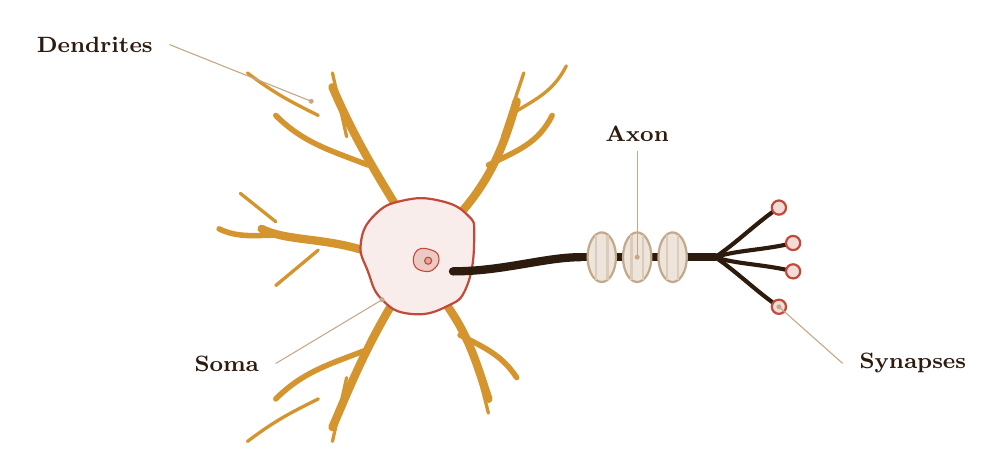
\begin{tikzpicture}[scale=0.9, >=latex]
    % Dendrites (Drawn first so they tuck under the Soma)
    % Dendrite 1 (Upper Right)
    \draw[wp-accent, line width=3pt, line cap=round] (0.4, 0.4) .. controls (1.0, 1.0) and (1.2, 1.5) .. (1.4, 2.2);
    \draw[wp-accent, line width=2pt, line cap=round] (1.0, 1.3) .. controls (1.4, 1.5) and (1.7, 1.6) .. (1.9, 2.0);
    \draw[wp-accent, line width=1.2pt, line cap=round] (1.2, 1.7) -- (1.5, 2.6);
    \draw[wp-accent, line width=1.2pt, line cap=round] (1.3, 2.0) .. controls (1.6, 2.2) and (1.9, 2.3) .. (2.1, 2.7);
    
    % Dendrite 2 (Upper Left)
    \draw[wp-accent, line width=3pt, line cap=round] (-0.1, 0.4) .. controls (-0.6, 1.2) and (-0.9, 1.7) .. (-1.2, 2.4);
    \draw[wp-accent, line width=2pt, line cap=round] (-0.7, 1.3) .. controls (-1.2, 1.5) and (-1.6, 1.6) .. (-2.0, 2.0);
    \draw[wp-accent, line width=1.2pt, line cap=round] (-1.0, 1.7) -- (-1.2, 2.6);
    \draw[wp-accent, line width=1.2pt, line cap=round] (-1.4, 2.0) .. controls (-1.8, 2.2) and (-2.0, 2.3) .. (-2.4, 2.6);
    
    % Dendrite 3 (Left)
    \draw[wp-accent, line width=3pt, line cap=round] (-0.5, 0) .. controls (-1.2, 0.3) and (-1.8, 0.2) .. (-2.2, 0.4);
    \draw[wp-accent, line width=2pt, line cap=round] (-1.6, 0.25) .. controls (-2.0, 0.4) and (-2.4, 0.2) .. (-2.8, 0.4);
    \draw[wp-accent, line width=1.2pt, line cap=round] (-2.0, 0.5) -- (-2.5, 0.9);
    \draw[wp-accent, line width=1.2pt, line cap=round] (-1.4, 0.1) -- (-2.0, -0.4);
    
    % Dendrite 4 (Lower Left)
    \draw[wp-accent, line width=3pt, line cap=round] (-0.2, -0.4) .. controls (-0.7, -1.2) and (-0.9, -1.7) .. (-1.2, -2.4);
    \draw[wp-accent, line width=2pt, line cap=round] (-0.7, -1.3) .. controls (-1.2, -1.5) and (-1.6, -1.6) .. (-2.0, -2.0);
    \draw[wp-accent, line width=1.2pt, line cap=round] (-1.0, -1.7) -- (-1.2, -2.6);
    \draw[wp-accent, line width=1.2pt, line cap=round] (-1.4, -2.0) .. controls (-1.8, -2.2) and (-2.0, -2.3) .. (-2.4, -2.6);
    
    % Dendrite 5 (Lower Right)
    \draw[wp-accent, line width=3pt, line cap=round] (0.2, -0.4) .. controls (0.7, -1.0) and (0.8, -1.4) .. (1.0, -2.0);
    \draw[wp-accent, line width=2pt, line cap=round] (0.6, -1.1) .. controls (1.0, -1.3) and (1.2, -1.4) .. (1.4, -1.7);
    \draw[wp-accent, line width=1.2pt, line cap=round] (0.8, -1.4) -- (1.0, -2.2);
    
    % Soma (Cell Body) - Organic irregular shape
    \draw[draw=wp-primary, fill=wp-primary!10, thick] plot [smooth cycle, tension=0.8] coordinates {
        (0.8, 0.3) (0.7, 0.6) (0.3, 0.8) (-0.2, 0.8) (-0.6, 0.6) (-0.8, 0.2) (-0.7, -0.2) (-0.5, -0.6) (-0.1, -0.8) (0.4, -0.7) (0.7, -0.4)
    };
    
    % Nucleus & Nucleolus
    \draw[draw=wp-primary, fill=wp-primary!30] plot [smooth cycle, tension=0.8] coordinates {
        (0.2, 0.1) (0.3, 0) (0.25, -0.15) (0.1, -0.2) (-0.05, -0.1) (0, 0.1)
    };
    \draw[draw=wp-primary, fill=wp-primary!50] (0.15, -0.05) circle (0.05cm);
    
    % Axon - Curves gracefully out of the Soma
    \draw[wp-text, line width=3pt, line cap=round] (0.5, -0.2) .. controls (1.2, -0.2) and (1.8, 0) .. (2.3, 0);
    \draw[wp-text, line width=3pt, line cap=round] (2.3, 0) -- (4.2, 0);
    
    % Myelin Sheath - With subtle inner lines for lipid bilayer texture
    \foreach \x in {2.6, 3.1, 3.6} {
        \draw[draw=wp-muted, fill=wp-muted!30, thick] (\x, 0) ellipse (0.2cm and 0.35cm);
        \draw[wp-muted!60, thick] (\x-0.08, 0.32) -- (\x-0.08, -0.32);
        \draw[wp-muted!60, thick] (\x+0.08, 0.32) -- (\x+0.08, -0.32);
    }
    
    % Axon Terminals (Synapses)
    \begin{scope}[shift={(4.2, 0)}]
        \draw[wp-text, line width=1.5pt, line cap=round] (0,0) .. controls (0.3, 0.2) and (0.6, 0.5) .. (0.9, 0.7);
        \draw[wp-text, line width=1.5pt, line cap=round] (0,0) .. controls (0.3, 0.1) and (0.7, 0.1) .. (1.1, 0.2);
        \draw[wp-text, line width=1.5pt, line cap=round] (0,0) .. controls (0.3, -0.1) and (0.7, -0.1) .. (1.1, -0.2);
        \draw[wp-text, line width=1.5pt, line cap=round] (0,0) .. controls (0.3, -0.2) and (0.6, -0.5) .. (0.9, -0.7);
        
        \foreach \pos in {(0.9, 0.7), (1.1, 0.2), (1.1, -0.2), (0.9, -0.7)} {
            \draw[draw=wp-primary, fill=wp-primary!20, thick] \pos circle (0.1cm);
        }
    \end{scope}

    % ==========================================
    % MODERN SCHEMATIC ANNOTATIONS (Leader Lines)
    % ==========================================
    
    % Dendrites Label
    \fill[wp-muted] (-1.5, 2.2) circle (1pt);
    \draw[wp-muted, thin] (-1.5, 2.2) -- (-3.5, 3.0);
    \node[font=\footnotesize\bfseries, wp-text, anchor=east] at (-3.6, 3.0) {Dendrites};
    
    % Soma Label
    \fill[wp-muted] (-0.5, -0.6) circle (1pt);
    \draw[wp-muted, thin] (-0.5, -0.6) -- (-2.0, -1.5);
    \node[font=\footnotesize\bfseries, wp-text, anchor=east] at (-2.1, -1.5) {Soma};
    
    % Axon Label
    \fill[wp-muted] (3.1, 0) circle (1pt);
    \draw[wp-muted, thin] (3.1, 0) -- (3.1, 1.5);
    \node[font=\footnotesize\bfseries, wp-text, anchor=south] at (3.1, 1.5) {Axon};
    
    % Synapses Label
    \fill[wp-muted] (5.1, -0.7) circle (1pt);
    \draw[wp-muted, thin] (5.1, -0.7) -- (6.0, -1.5);
    \node[font=\footnotesize\bfseries, wp-text, anchor=west] at (6.1, -1.5) {Synapses};
    
\end{tikzpicture}}
\caption{Anatomy of a biological neuron. Electrical signals flow from dendrites, through the soma, down the axon, to the synapses.}
\label{fig:bio_neuron}
\end{figure}

\subsection{Anatomy of a Neuron}

A biological neuron is a specialized cell that processes and transmits electrical and chemical signals. It consists of three main structural components:

\begin{enumerate}[leftmargin=*, itemsep=4pt]
    \item \textbf{Dendrites:} These are tree-like extensions that act as the "antennae" of the neuron. They receive signals (neurotransmitters) from other neurons. The physical structure of the dendrites determines how the neuron integrates these incoming signals.
    \item \textbf{Soma (Cell Body):} The soma contains the nucleus of the cell. Its critical function is to aggregate the electrical signals received from the dendrites. It acts as an integrator, summing up the excitatory and inhibitory inputs.
    \item \textbf{Axon:} If the aggregated signal in the soma exceeds a certain threshold, the neuron "fires." This generates an electrical impulse called an action potential, which travels down the axon. The axon is the output wire of the neuron.
    \item \textbf{Synapses:} At the end of the axon are terminal branches that form connections (synapses) with the dendrites of other neurons. The \textit{strength} of these synaptic connections determines how much influence one neuron has on another. 
\end{enumerate}

\subsection{The Action Potential and Non-Linearity}

A crucial biological feature is how the neuron decides to fire. The soma does not simply pass along the sum of its inputs linearly. Instead, it operates on an "all-or-nothing" principle.

When the aggregated electrical potential inside the cell reaches a specific \textit{threshold}, voltage-gated ion channels open, causing a massive, rapid spike in voltage—the action potential. If the input is below the threshold, nothing happens; the neuron remains silent.

Furthermore, the strength of the connections (synapses) is not fixed. Biological synapses exhibit \textbf{plasticity}. If two neurons fire together frequently, the synaptic connection between them strengthens. This is known as Hebbian theory: "Neurons that fire together, wire together." This biological adaptation of connection strengths is the direct inspiration for how artificial neural networks "learn" by adjusting weights.

\section{From Biology to Mathematics: The Artificial Neuron}

In the 1940s and 1950s, researchers like Warren McCulloch and Walter Pitts sought to abstract the biological neuron into a mathematical model. They recognized that the structural components of a biological neuron could be translated into algebraic operations.

\begin{table}[h]
\centering
\begin{adjustbox}{max width=\textwidth}
\begin{tabular}{@{}lll@{}}
\toprule
\textbf{Biological Concept} & \textbf{Mathematical Abstraction} & \textbf{Symbol} \\ \midrule
Dendrites (receiving signals) & Input vector & $\mathbf{x}$ \\
Synaptic strength & Weight parameter & $\mathbf{w}$ \\
Soma (signal integration) & Dot product (weighted sum) & $\mathbf{w} \cdot \mathbf{x}$ \\
Baseline firing threshold & Bias parameter & $b$ \\
Action Potential (all-or-nothing) & Non-linear activation function & $\phi(\cdot)$ \\ \bottomrule
\end{tabular}
\end{adjustbox}
\caption{Mapping biological mechanisms to the mathematical components of an artificial neuron.}
\label{tab:bio_to_math}
\end{table}

A single artificial neuron (historically called a Perceptron) is fundamentally an affine transformation followed by a non-linear function. It maps an input vector $\mathbf{x} = (x_1,\dots,x_d)^{\mathsf{T}} \in \mathbb{R}^d$ to an output $o$:

 $$ o = \phi(\mathbf{w} \cdot \mathbf{x} + b)
 $$ 
Here, the parameters $\theta$ are the weights $\mathbf{w} \in \mathbb{R}^d$ and the bias $b \in \mathbb{R}$. But what does the operation $\mathbf{w} \cdot \mathbf{x}$ actually represent? 

Geometrically, the dot product is a measure of \textit{alignment} between two vectors. If the input vector $\mathbf{x}$ points in a similar direction to the weight vector $\mathbf{w}$, their dot product is a large positive number. If they point in opposite directions, it is negative. If they are perpendicular, it is zero. Therefore, the weights act as a \textit{filter}: the neuron outputs a high value only when the input matches a specific pattern encoded in $\mathbf{w}$.

The bias $b$ acts as a baseline threshold. It shifts the activation point, allowing the neuron to fire even when the alignment with $\mathbf{w}$ is not perfectly positive, or requiring a very strong alignment to fire at all.

Geometrically, the weights define a hyperplane that cuts the space. A single neuron can only represent \textit{linearly separable} functions; the XOR problem is the classic counterexample where no single hyperplane can partition the activation states.
\begin{figure}[htbp]
\centering
\begin{subfigure}{0.48\textwidth}
    \centering
    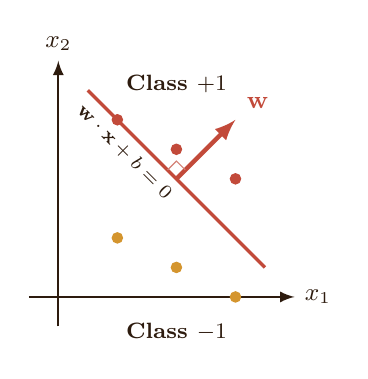
\begin{tikzpicture}[scale=0.75, >=latex]
        \draw[->, thick, wp-text] (-0.5,0) -- (4,0) node[right, font=\small\bfseries]{$x_1$};
        \draw[->, thick, wp-text] (0,-0.5) -- (0,4) node[above, font=\small\bfseries]{$x_2$};
        \draw[wp-primary, very thick] (0.5,3.5) -- (3.5,0.5);
        \node[wp-text, font=\scriptsize\bfseries, below left, rotate=-45] at (2.2,1.8) {$\mathbf{w}\cdot\mathbf{x}+b=0$};
        \coordinate (origen_w) at (2,2);
        \draw[->, wp-primary, ultra thick] (origen_w) -- ++(1,1) node[above right, font=\small\bfseries] {$\mathbf{w}$};
        \draw[wp-primary!70, thin] (2,2) ++(0.15,0.15) -- ++(-0.15,0.15) -- ++(-0.15,-0.15);
        \filldraw[wp-primary] (1,3) circle (2.5pt);
        \filldraw[wp-primary] (2,2.5) circle (2.5pt);
        \filldraw[wp-primary] (3,2) circle (2.5pt);
        \filldraw[wp-accent] (1,1) circle (2.5pt);
        \filldraw[wp-accent] (2,0.5) circle (2.5pt);
        \filldraw[wp-accent] (3,0) circle (2.5pt);
        \node[wp-text, font=\footnotesize\bfseries] at (2.0,3.6) {Class $+1$};
        \node[wp-text, font=\footnotesize\bfseries] at (2.0,-0.6) {Class $-1$};
    \end{tikzpicture}
    \caption{Linear boundary}
    \label{fig:cartesian_boundary}
\end{subfigure}\hfill
\begin{subfigure}{0.48\textwidth}
    \centering
    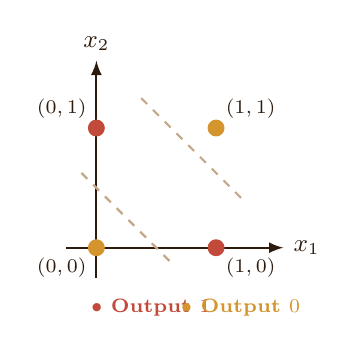
\begin{tikzpicture}[scale=0.95, >=latex]
        \draw[->, thick, wp-text] (-0.4,0) -- (2.5,0) node[right, font=\small\bfseries]{$x_1$};
        \draw[->, thick, wp-text] (0,-0.4) -- (0,2.5) node[above, font=\small\bfseries]{$x_2$};
        \filldraw[wp-accent] (0,0) circle (3pt);
        \node[wp-text, font=\scriptsize\bfseries, below left] at (0,0) {$(0,0)$};
        \filldraw[wp-accent] (1.6,1.6) circle (3pt);
        \node[wp-text, font=\scriptsize\bfseries, above right] at (1.6,1.6) {$(1,1)$};
        \filldraw[wp-primary] (1.6,0) circle (3pt);
        \node[wp-text, font=\scriptsize\bfseries, below right] at (1.6,0) {$(1,0)$};
        \filldraw[wp-primary] (0,1.6) circle (3pt);
        \node[wp-text, font=\scriptsize\bfseries, above left] at (0,1.6) {$(0,1)$};
        \draw[dashed, wp-muted, thick] (-0.2,1.0) -- (1.0,-0.2);
        \draw[dashed, wp-muted, thick] (0.6,2.0) -- (2.0,0.6);
        \node[wp-primary, font=\scriptsize\bfseries, anchor=west] at (-0.2,-0.8) {$\bullet$ Output $1$};
        \node[wp-accent, font=\scriptsize\bfseries, anchor=west] at (1.0,-0.8) {$\bullet$ Output $0$};
    \end{tikzpicture}
    \caption{XOR dilemma}
    \label{fig:xor_problem}
\end{subfigure}
\caption{Geometric representation of linear separability. (a) A single hyperplane partitions space based on the weight vector $\mathbf{w}$. (b) The XOR problem cannot be solved by a single linear hyperplane.}
\label{fig:linear_vs_xor}
\end{figure}

\begin{lstlisting}[caption={Implementing the Neuron class in \texttt{mini\_nn/primitives.py}.}]
import numpy as np

class Neuron:
    def __init__(self, in_dim):
        # Random initialization for the forward pass
        self.w = np.random.randn(in_dim)
        self.b = np.random.randn()
        
    def __call__(self, x):
        # Affine transformation: w * x + b
        z = np.dot(self.w, x) + self.b
        # Non-linear activation (ReLU)
        return np.maximum(0, z)
\end{lstlisting}

\subsection{Activation Functions}

For multilayer networks, we need nonlinear, differentiable activation functions. Without them, stacking layers would merely result in a single linear transformation ($\mathbf{W}_2(\mathbf{W}_1\mathbf{x}) = \mathbf{W}'\mathbf{x}$). 

\begin{figure}[h]
\centering
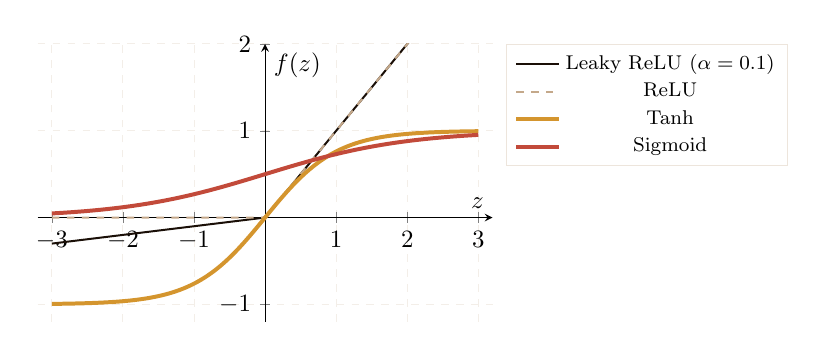
\begin{tikzpicture}[scale=0.9, thick]
    \begin{axis}[
        width=8cm, height=5.5cm,
        xlabel={$z$},
        ylabel={$f(z)$},
        domain=-3:3,
        samples=150,
        axis lines=middle,
        ymin=-1.2, ymax=2.0,
        xmin=-3.2, xmax=3.2,
        grid=major,
        grid style={dashed, wp-muted!20},
        legend pos=outer north east,
        legend style={font=\footnotesize, draw=wp-muted!30}
    ]
        \addplot[wp-dark, thick] {max(0.1*x,x)};
        \addplot[wp-muted, thick, dashed] {max(0,x)};
        \addplot[wp-accent, ultra thick] {tanh(x)};
        \addplot[wp-primary, ultra thick] {1 / (1 + exp(-x))};
        \legend{Leaky ReLU ($\alpha=0.1$), ReLU, Tanh, Sigmoid}
    \end{axis}
\end{tikzpicture}
\caption{Common activation functions. Sigmoid and tanh saturate at the tails, causing gradients to vanish. ReLU is piecewise linear, preserving gradients for positive inputs.}
\label{fig:activations}
\end{figure}

Geometrically, linear transformations ($\mathbf{W}\mathbf{x}$) only stretch, rotate, or shear the space. Activation functions are responsible for \textit{bending} or \textit{folding} the space. The Rectified Linear Unit (ReLU), defined as $\max(0, z)$, acts like origami: it folds the negative quadrants of the space onto the boundaries of the positive ones, allowing the network to carve complex decision boundaries out of the input space.

\subsection{Multilayer Perceptron (MLP)}

To solve non-linear problems like XOR, we stack multiple layers of neurons. A multilayer perceptron (MLP) consists of an input layer, one or more hidden layers, and an output layer. 

Instead of computing neurons one by one, we use linear algebra to compute an entire layer simultaneously. Let $\mathbf{o}^{(\ell-1)} \in \mathbb{R}^{d_{in}}$ be the output of the previous layer. We define a weight matrix $\mathbf{W}^{(\ell)} \in \mathbb{R}^{d_{out} \times d_{in}}$ and a bias vector $\mathbf{b}^{(\ell)} \in \mathbb{R}^{d_{out}}$. The forward pass for layer $\ell$ is:
\[
\mathbf{a}^{(\ell)} = \mathbf{W}^{(\ell)}\mathbf{o}^{(\ell-1)} + \mathbf{b}^{(\ell)},\qquad 
\mathbf{o}^{(\ell)} = f^{(\ell)}(\mathbf{a}^{(\ell)}),
\]
where each \textit{row} of $\mathbf{W}^{(\ell)}$ corresponds to the weights of a single neuron in the new layer. The matrix multiplication efficiently computes the dot products of all neurons against the input simultaneously.


\begin{lstlisting}[caption={Implementing the Layer and MLP classes in \texttt{mini\_nn/layers.py}.}]
class Layer:
    def __init__(self, in_dim, out_dim):
        self.W = np.random.randn(out_dim, in_dim)
        self.b = np.random.randn(out_dim)
        
    def __call__(self, x):
        # Affine transformation for a single input vector x (a column of a batch)
        z = np.dot(self.W, x) + self.b
        return np.maximum(0, z) # ReLU activation

class MLP:
    def __init__(self, sizes):
        # sizes: [in_dim, hidden_1, hidden_2, ..., out_dim]
        self.layers = [Layer(sizes[i], sizes[i+1]) 
                       for i in range(len(sizes)-1)]
        
    def __call__(self, x):
        for layer in self.layers:
            x = layer(x) # Forward pass sequentially
        return x
\end{lstlisting}

\begin{remark}[Bridge to Chapter 2]
This chapter implements the \emph{forward pass} using plain numpy: the weights $\mathbf{W}$ are static arrays, and the network cannot improve its predictions. In Chapter 2 we will replace these arrays with \texttt{Valor}---a tiny automatic-differentiation engine---so that each weight becomes a differentiable node of a computational graph. The forward computation stays exactly the same (affine transformation followed by an activation); the only difference is that every operation now records how it was computed, enabling the backward pass that makes the network trainable. The \texttt{mini\_nn} framework is thus upgraded in place: same architecture, differentiable core.
\end{remark}
\subsection{Measuring the Error: Loss Functions}

Once the network produces an output $\hat{\mathbf{y}} = \mathbf{o}^{(L)}$, we need a mechanism to measure how far it is from the target $\mathbf{t}$. This is the role of the \textbf{Loss Function} $\mathcal{L}(\hat{\mathbf{y}}, \mathbf{t})$. The choice of loss function dictates how the network penalizes mistakes.

\subsubsection{Mean Squared Error (MSE)}
For regression tasks (predicting continuous numbers), we want to penalize the distance between the prediction and the target. We use the squared error:
\[
\mathcal{L}_{\text{MSE}} = \frac{1}{2}\|\mathbf{t} - \hat{\mathbf{y}}\|^2
\]
Why square it? First, it ensures the error is always positive. Second, it heavily penalizes large errors (being off by 10 costs 100, while being off by 1 costs 1), which encourages the network to fix its worst mistakes first.

\subsubsection{Cross-Entropy Loss}
For classification tasks, the network outputs raw scores called \textit{logits}. We first use the Softmax function to squash these into probabilities that sum to 1:
\[
\text{Softmax}(\hat{y}_i) = \frac{e^{\hat{y}_i}}{\sum_j e^{\hat{y}_j}}
\]
To measure the error, we use Cross-Entropy. Unlike MSE, Cross-Entropy punishes the network exponentially if it is \textit{confident but wrong}. If the true class is $i$, the loss is:
\[
\mathcal{L}_{\text{CE}} = -\log(\text{Softmax}(\hat{y}_i))
\]
If the network predicts a probability of $0.99$ for the true class, $\mathcal{L} \approx 0.01$. If it predicts $0.01$, $\mathcal{L} \approx 4.6$. This steep penalty forces the network to learn the correct class boundaries quickly.

\subsection{Universal Approximation Theorem}

\begin{thm}[Cybenko, 1989]
    Let $\sigma: \mathbb{R}\to\mathbb{R}$ be a continuous, bounded, non-constant activation function. Then for any continuous function $f: [0,1]^d \to \mathbb{R}$ and any $\varepsilon>0$, there exist $N\in\mathbb{N}$, vectors $\mathbf{w}_j\in\mathbb{R}^d$, scalars $v_j, b_j\in\mathbb{R}$ such that
    \[
    \sup_{\mathbf{x}\in[0,1]^d} \left| \sum_{j=1}^N v_j\,\sigma(\mathbf{w}_j\cdot\mathbf{x} + b_j) - f(\mathbf{x}) \right| < \varepsilon.
    \]
\end{thm}

The theorem guarantees that the hypothesis space of an MLP (with enough neurons) contains a function that can approximate any continuous function arbitrarily well. This proves that our architectural components possess the mathematical capacity to model complex phenomena. However, the theorem says nothing about \textit{how} to find those parameters $\theta$.

\begin{figure}[htbp]
\centering
\resizebox{\textwidth}{!}{%
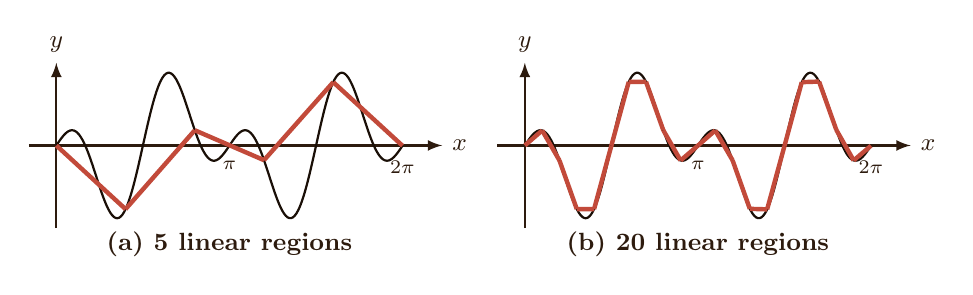
\begin{tikzpicture}[scale=0.7, >=latex, thick]
    % --- First plot: 5 linear regions ---
    \begin{scope}[shift={(0, 0)}]
        % Draw axes
        \draw[->, wp-text] (-0.5, 0) -- (7, 0) node[right, font=\small] {$x$};
        \draw[->, wp-text] (0, -1.5) -- (0, 1.5) node[above, font=\small] {$y$};
        
        % Draw the noisy target function
        \draw[wp-dark, thick, domain=0:6.28, samples=200, smooth] 
            plot (\x, {1.5 * sin(\x r) * cos(3*\x r)});

        % Draw linear approximation automatically with 5 regions
        \foreach \i in {0,...,4} {
            \pgfmathsetmacro{\xstart}{\i * 6.28 / 5}
            \pgfmathsetmacro{\xend}{(\i + 1) * 6.28 / 5}
            \pgfmathsetmacro{\ystart}{1.5 * sin(\xstart r) * cos(3*\xstart r)}
            \pgfmathsetmacro{\yend}{1.5 * sin(\xend r) * cos(3*\xend r)}
            \draw[wp-primary, ultra thick] (\xstart, \ystart) -- (\xend, \yend);
        }

        % Axis labels
        \node[below, font=\scriptsize, wp-text] at (3.14, -0.1) {$\pi$};
        \node[below, font=\scriptsize, wp-text] at (6.28, -0.1) {$2\pi$};
        \node[wp-text, font=\small\bfseries] at (3.14, -1.8) {(a) 5 linear regions};
    \end{scope}

    % --- Second plot: 20 linear regions ---
    \begin{scope}[shift={(8.5, 0)}]
        % Draw axes
        \draw[->, wp-text] (-0.5, 0) -- (7, 0) node[right, font=\small] {$x$};
        \draw[->, wp-text] (0, -1.5) -- (0, 1.5) node[above, font=\small] {$y$};

        % Draw the noisy target function
        \draw[wp-dark, thick, domain=0:6.28, samples=200, smooth] 
            plot (\x, {1.5 * sin(\x r) * cos(3*\x r)});

        % Draw linear approximation automatically with 20 regions
        \foreach \i in {0,...,19} {
            \pgfmathsetmacro{\xstart}{\i * 6.28 / 20}
            \pgfmathsetmacro{\xend}{(\i + 1) * 6.28 / 20}
            \pgfmathsetmacro{\ystart}{1.5 * sin(\xstart r) * cos(3*\xstart r)}
            \pgfmathsetmacro{\yend}{1.5 * sin(\xend r) * cos(3*\xend r)}
            \draw[wp-primary, ultra thick] (\xstart, \ystart) -- (\xend, \yend);
        }

        % Axis labels
        \node[below, font=\scriptsize, wp-text] at (3.14, -0.1) {$\pi$};
        \node[below, font=\scriptsize, wp-text] at (6.28, -0.1) {$2\pi$};
        \node[wp-text, font=\small\bfseries] at (3.14, -1.8) {(b) 20 linear regions};
    \end{scope}
\end{tikzpicture}}
\caption{Visualization of the Universal Approximation Theorem. The dark curve is a highly oscillatory target function $f(x) = 1.5\sin(x)\cos(3x)$. The terracotta lines represent the piecewise linear approximation formed by a neural network. With only 5 regions (a), the network misses the internal fluctuations entirely. With 20 regions (b), the approximation becomes highly precise.}
\label{fig:UAT}
\end{figure}

\begin{remark}
    We have defined our hypothesis space ($f_\theta$) and our objective ($\mathcal{L}$). However, our \texttt{mini\_nn} model currently relies on random initialization; it has no mechanism to improve its predictions. In Chapter 2, we will solve this by introducing Differentiable Programming and the optimization algorithms used to find $\theta^*$.
\end{remark}

\end{document}